\chapter{Ausarbeitung}
\section{Aufgabe 1}
In diese Aufgabe wird die Navigationsl"osung f"ur Drohne mit einem loosely-coupled Kalmanfilter berechnet. Zuerst wird der Hebelarm vernachl"assigt. Die Trajektorie steht in \autoref{fig:noarm}, die Unterschied zur interne L"osung in \autoref{fig:intern_diff}.(Erst 40 Sekunden werden vernachl"assigt weil es keine interne L"osung w"ahrend diesem Zeitraum gibt)
\begin{figure}[htpb]\centering
		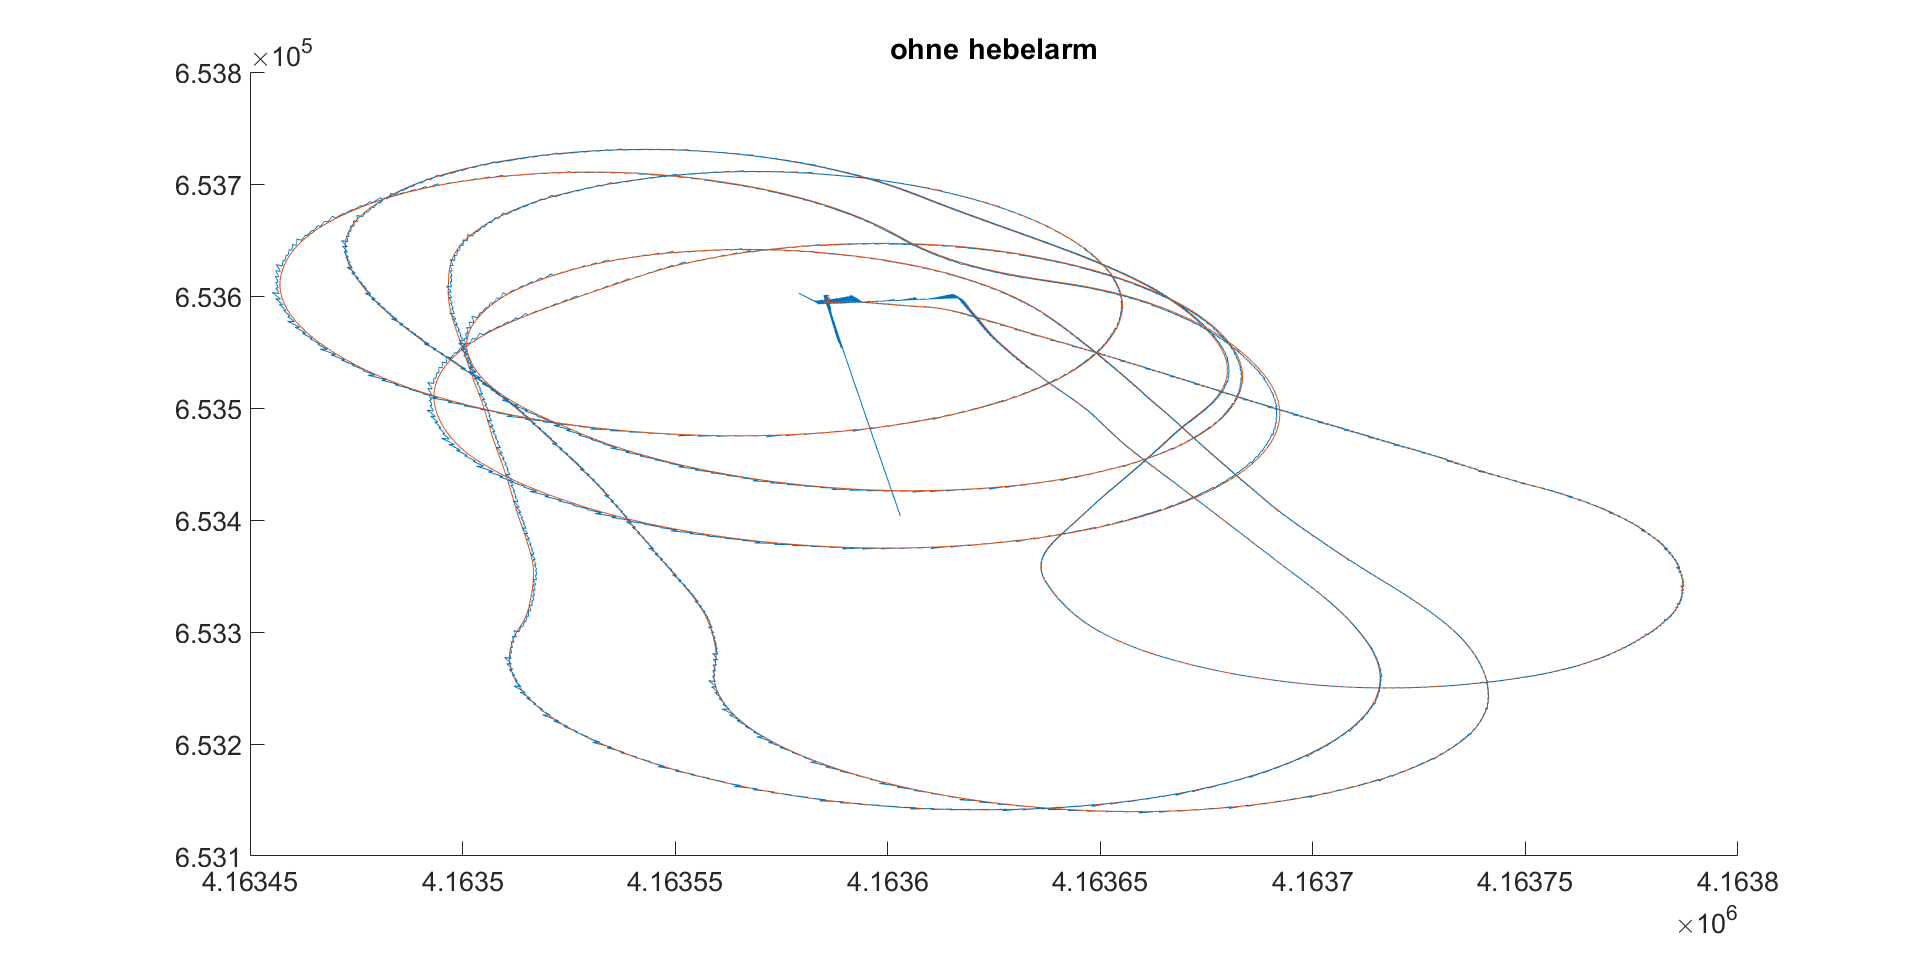
\includegraphics[width=0.9\textwidth]{tra_noarm.png}
		\caption{Trajektorie (Hebelarm vernachl"assigt)}
		\label{fig:noarm}
\end{figure}\\
\begin{figure}[htpb]\centering
	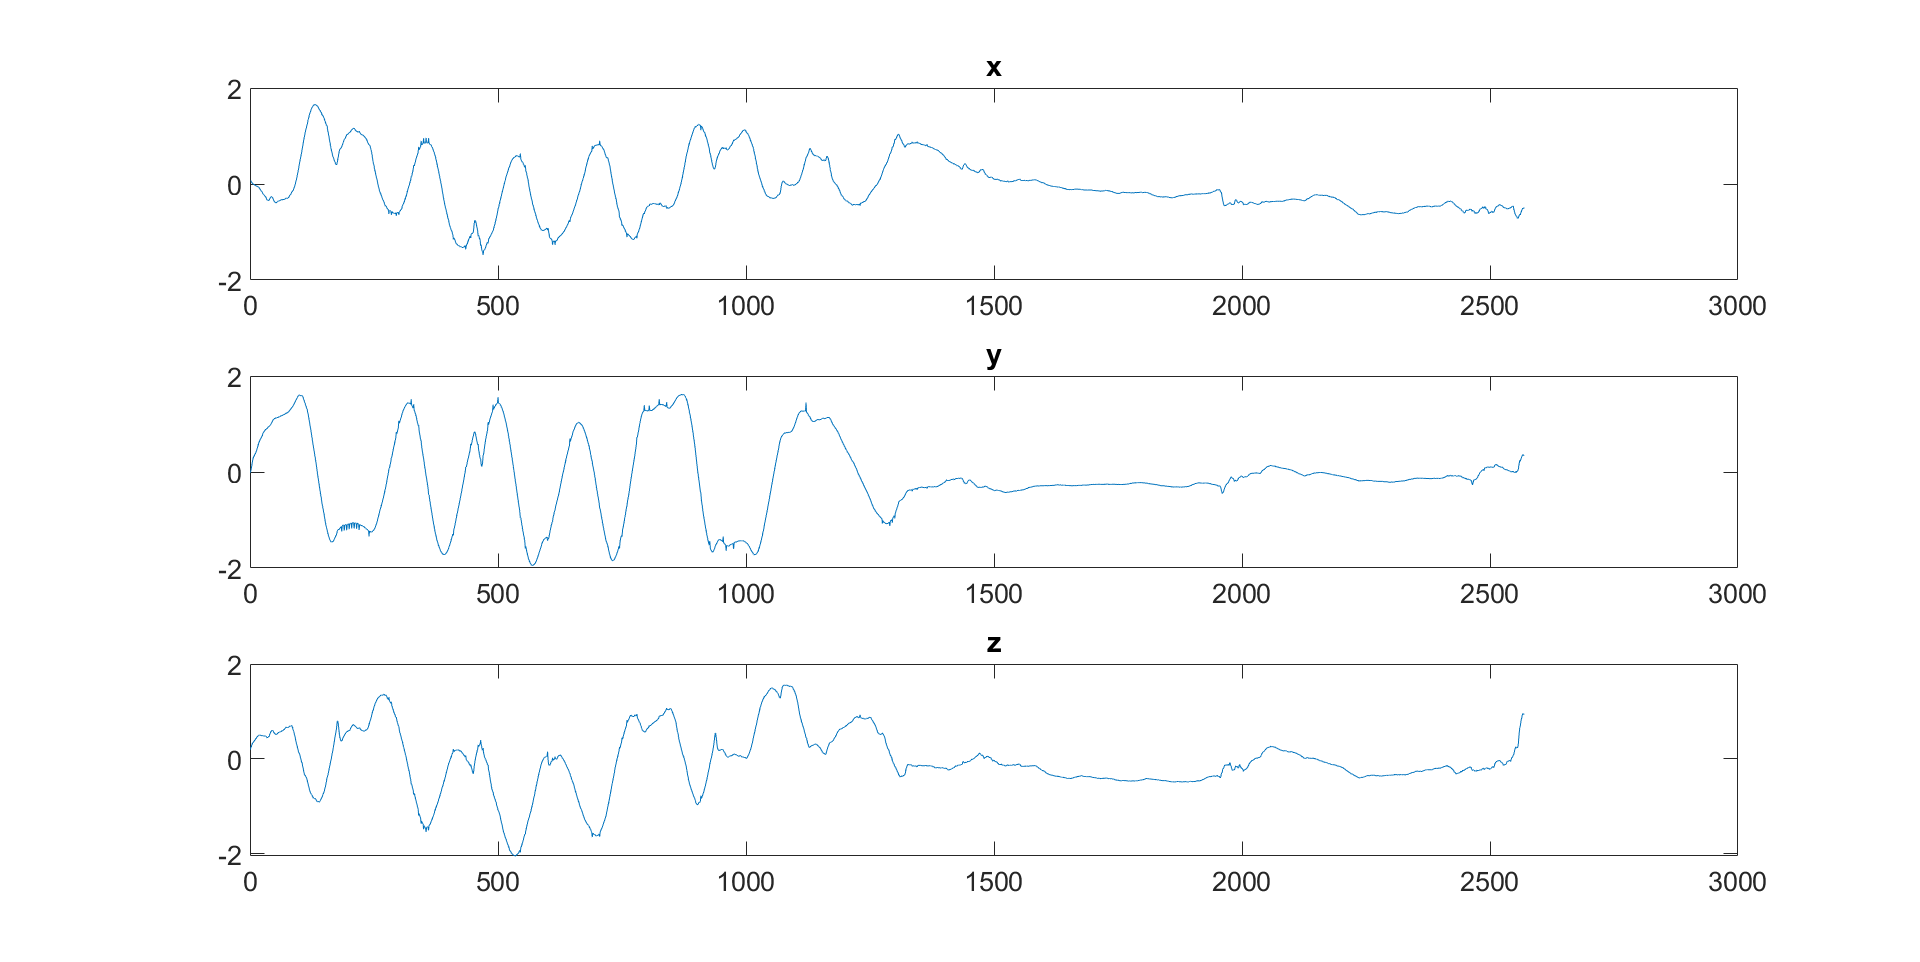
\includegraphics[width=0.9\textwidth]{intern_diff.png}
	\caption{Differenz mit Intern}
	\label{fig:intern_diff}
\end{figure}\\
Die Unterschied am Anfang sind relativ gr"o"ser um ca. 2m. Danach wird sie verkleinert. Die Fehler Zust"ande kann man von Hauptdiagonal der Varianz-Kovarianz Matrizen extrahieren. 
\clearpage
\section{Aufgabe 2}
Jetzt wird Hebelarm mitberechnet. Die Unterschied zwischen die Ergebnisse aus Aufgabe 1 und 2 liegt in \autoref{fig:diff2}. Die Unterschied in y-Richtung ist minimal weil beide der Mittelpunkt 2 GNSS Antenne und Imu System auf der Flugrichtungen liegt(x Achse in body system). In anderen Richtungen spielt Hebelarm eine Rolle, der Einfluss ist bei dem Fall klein weil der Arm kurz ist.
\begin{figure}[htpb]\centering
	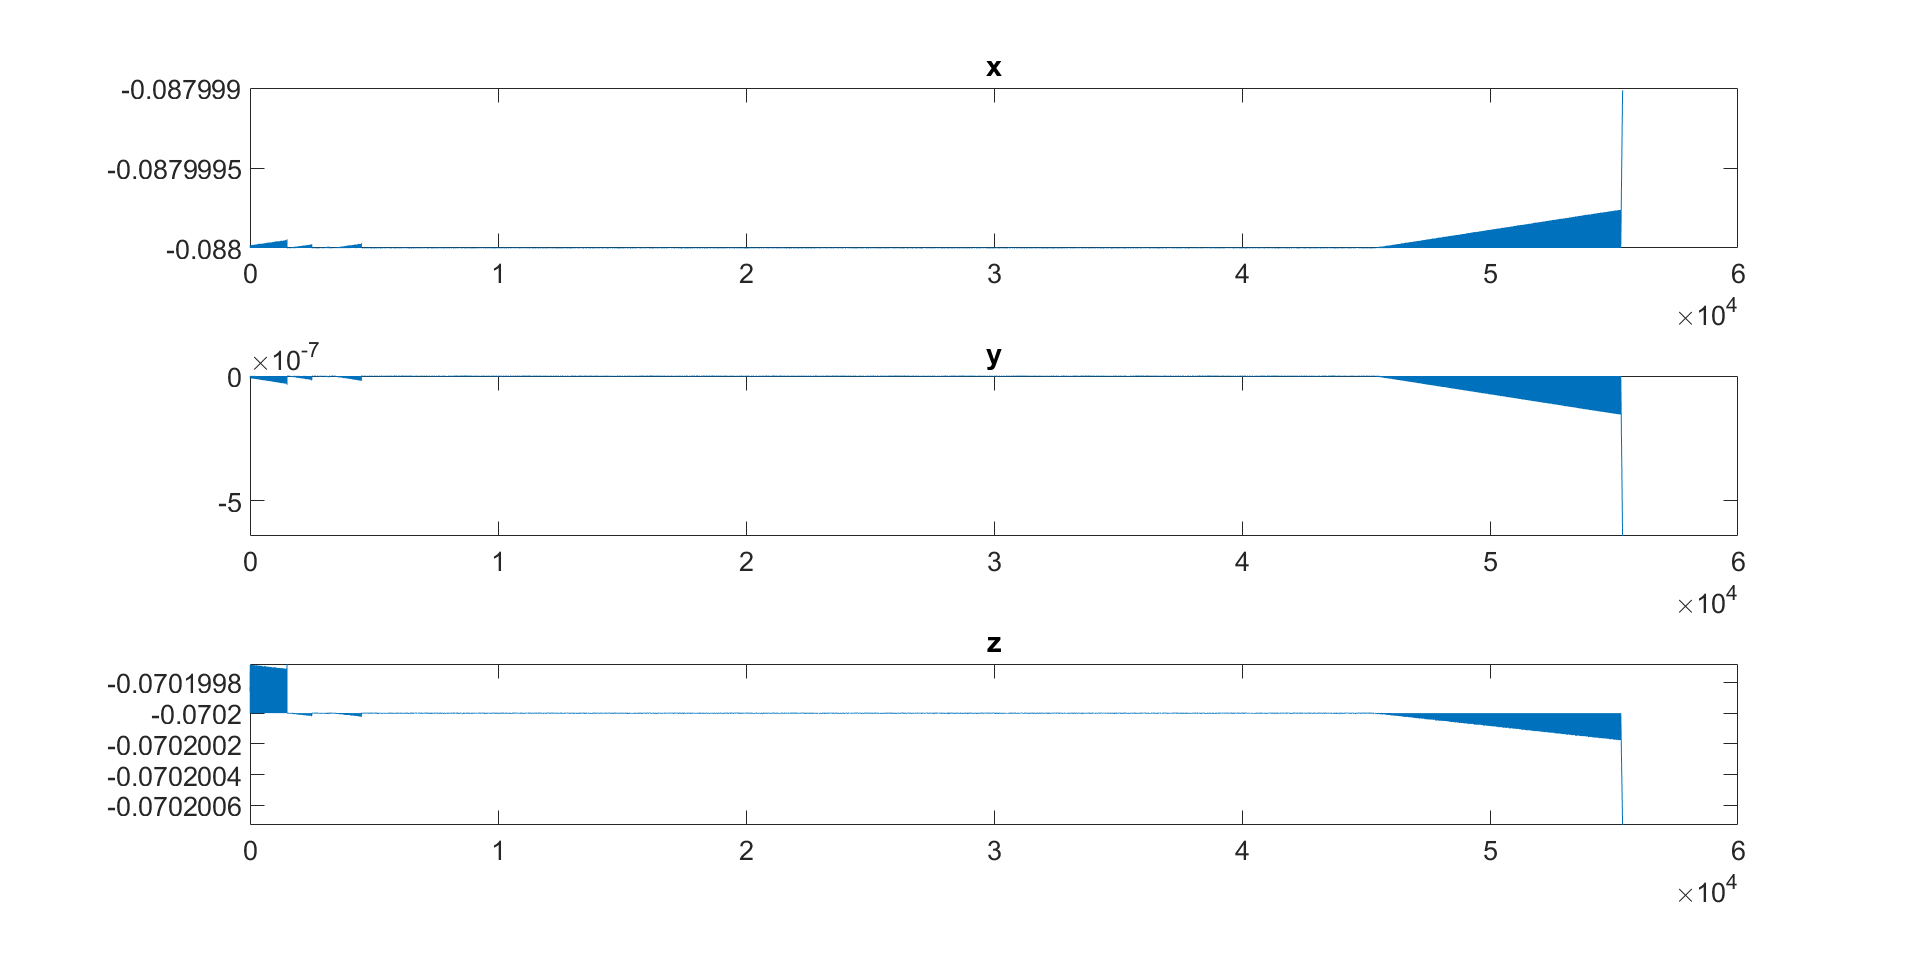
\includegraphics[width=0.9\textwidth]{diff2.png}
	\caption{Differenz}
	\label{fig:diff2}
\end{figure}\\
\begin{figure}[htpb]\centering
	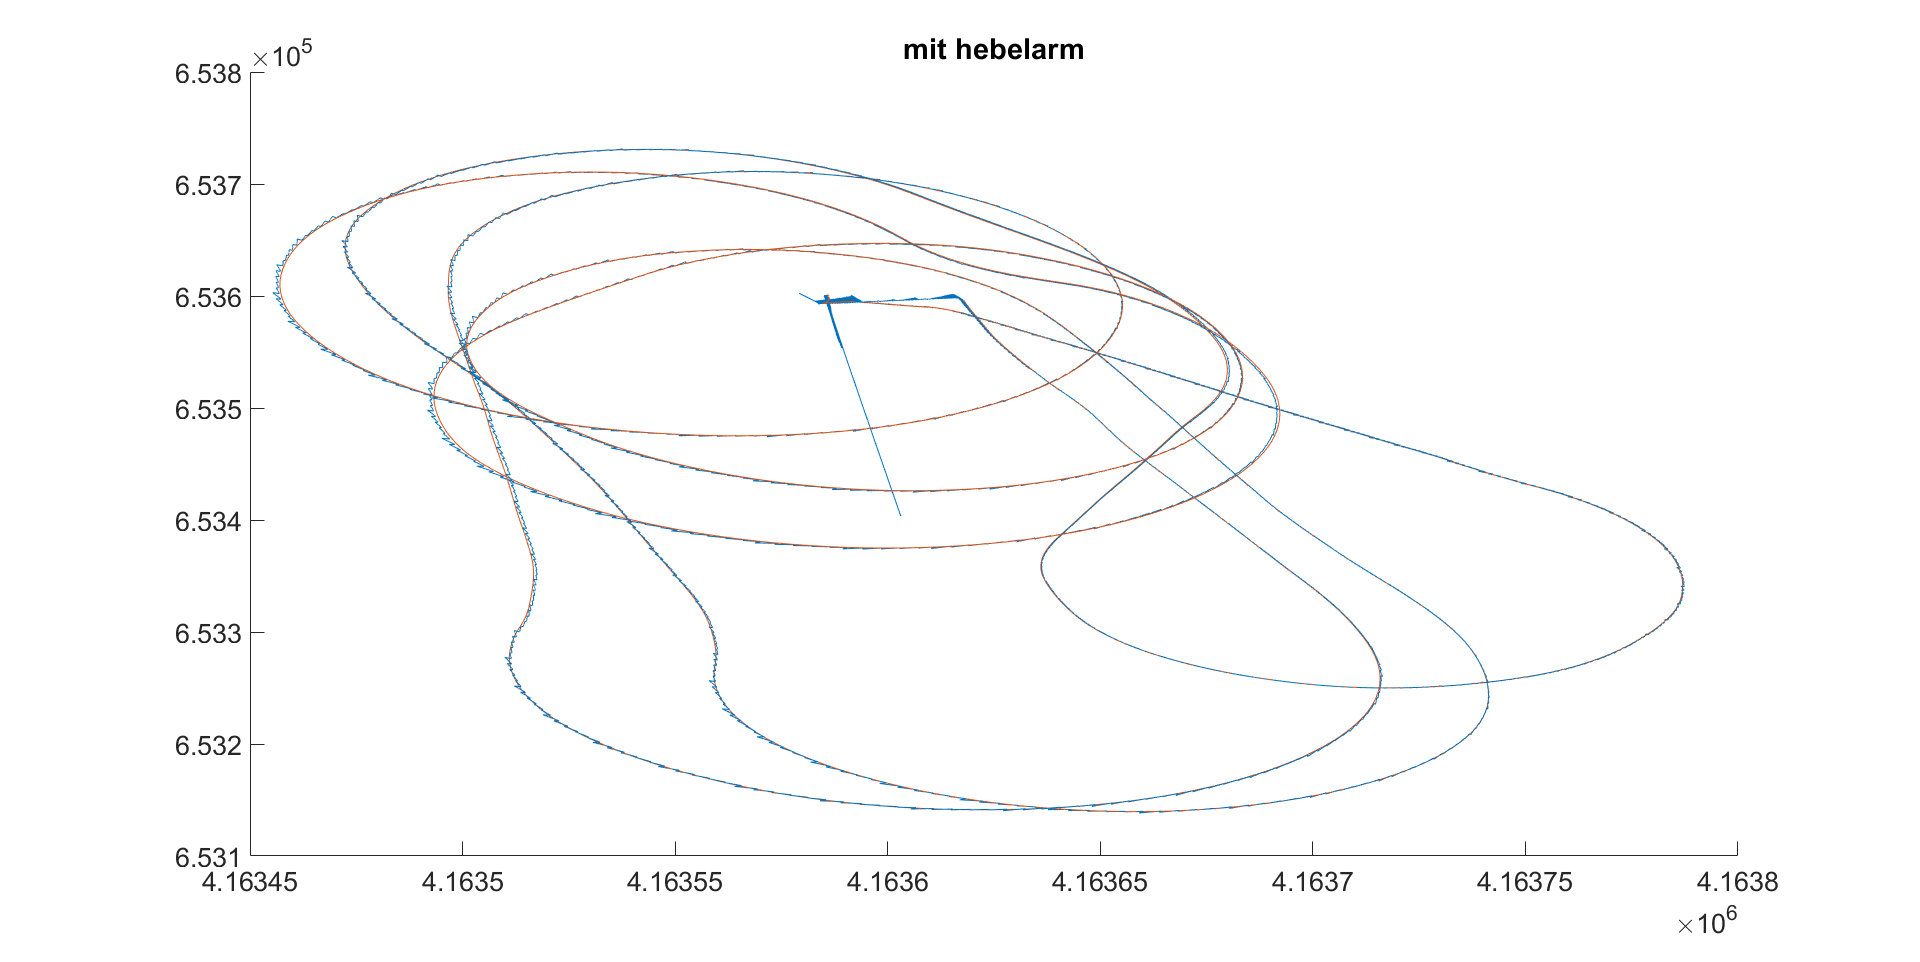
\includegraphics[width=0.9\textwidth]{tra_witharm.png}
	\caption{Trajektorie (Hebelarm)}
	\label{fig:arm}
\end{figure}
\clearpage
\lstset{language=Matlab,%
	%basicstyle=\color{red},
	breaklines=true,%
	morekeywords={matlab2tikz},
	keywordstyle=\color{blue},%
	morekeywords=[2]{1}, keywordstyle=[2]{\color{black}},
	identifierstyle=\color{black},%
	stringstyle=\color{purple},
	commentstyle=\color{green},%
	showstringspaces=false,%without this there will be a symbol in the places where there is a space
	numbers=left,%
	numberstyle={\tiny \color{black}},% size of the numbers
	numbersep=9pt, % this defines how far the numbers are from the text
	%emph=[2]{word1,word2}, emphstyle=[2]{style},    
}
\section{Matlab Code}
Die Code ist mit Ausarbeitung zusammen abgegeben.